%-------------------------------------------------------------------------------
%-------------------------------------------------------------------------------
\begin{frame}
\begin{itemize}
\item \bibentry{Keane.1997}
\end{itemize}
\end{frame}
%-------------------------------------------------------------------------------
%-------------------------------------------------------------------------------
\begin{frame}\begin{quote}
This paper provides structural estimates of a dynamic model of schooling, work, and occupational choice decisions ... The structural estimation framework that we adopt fully imposes the restrictions of the theory and permits an investigation of whether such a theoretically restricted model can succeed in quantitatively fitting the observed data patterns. We find that a suitably extended human capital investment model can in fact do an excellent job of fitting observed data ... and also produces reasonable forecasts of future work decisions and wage patterns.
\end{quote}\end{frame}

%-------------------------------------------------------------------------------
%-------------------------------------------------------------------------------
\begin{frame}[plain]
\begin{center}
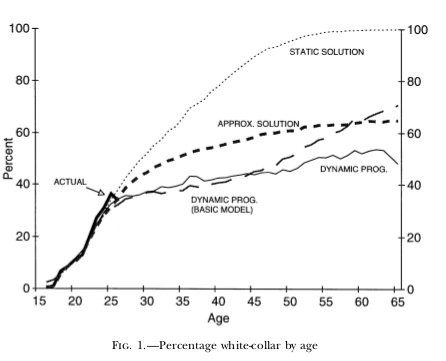
\includegraphics[width=.90\columnwidth]{fig-1}
\end{center}
\end{frame}
%-------------------------------------------------------------------------------
%-------------------------------------------------------------------------------
\begin{frame}[plain]
\begin{center}
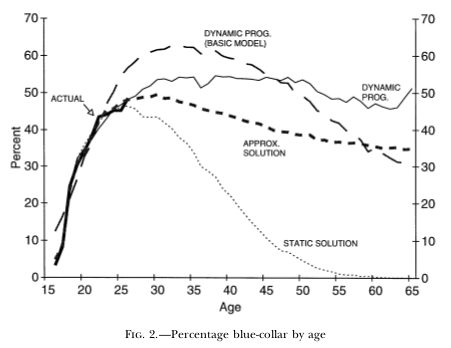
\includegraphics[width=.90\columnwidth]{fig-2}
\end{center}
\end{frame}
%-------------------------------------------------------------------------------
%-------------------------------------------------------------------------------
\begin{frame}[plain]
\begin{center}
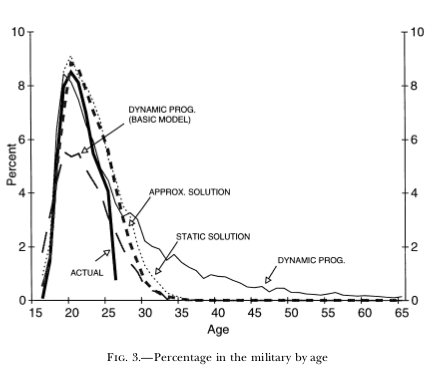
\includegraphics[width=.90\columnwidth]{fig-3}
\end{center}
\end{frame}
%-------------------------------------------------------------------------------
%-------------------------------------------------------------------------------
\begin{frame}[plain]
\begin{center}
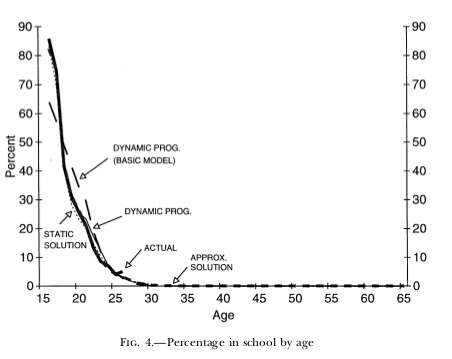
\includegraphics[width=.90\columnwidth]{fig-4}
\end{center}
\end{frame}
%-------------------------------------------------------------------------------
%-------------------------------------------------------------------------------
\begin{frame}[plain]
\begin{center}
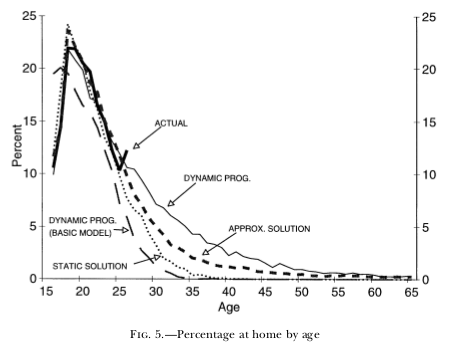
\includegraphics[width=.90\columnwidth]{fig-5}
\end{center}
\end{frame}
%-------------------------------------------------------------------------------
%-------------------------------------------------------------------------------
\begin{frame}[plain]
\begin{center}
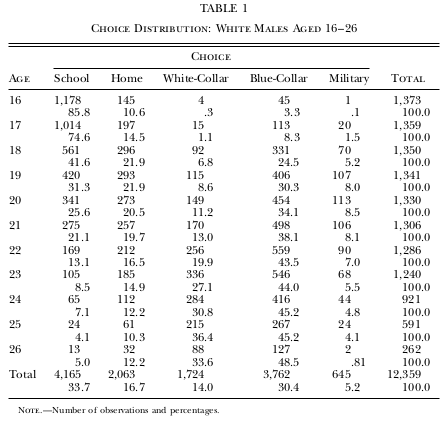
\includegraphics[width=.90\columnwidth]{tab-1}
\end{center}
\end{frame}
%-------------------------------------------------------------------------------
%-------------------------------------------------------------------------------
\begin{frame}[plain]
\begin{center}
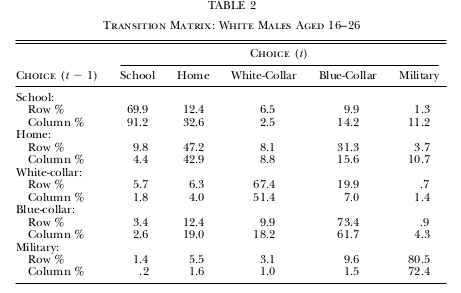
\includegraphics[width=.90\columnwidth]{tab-2}
\end{center}
\end{frame}
%-------------------------------------------------------------------------------
%-------------------------------------------------------------------------------
\begin{frame}[plain]
\begin{center}
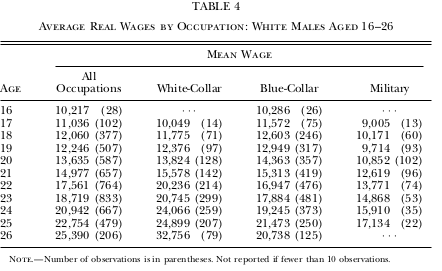
\includegraphics[width=.90\columnwidth]{tab-4}
\end{center}
\end{frame}
%-------------------------------------------------------------------------------
%-------------------------------------------------------------------------------
\begin{frame}[plain]
\begin{center}
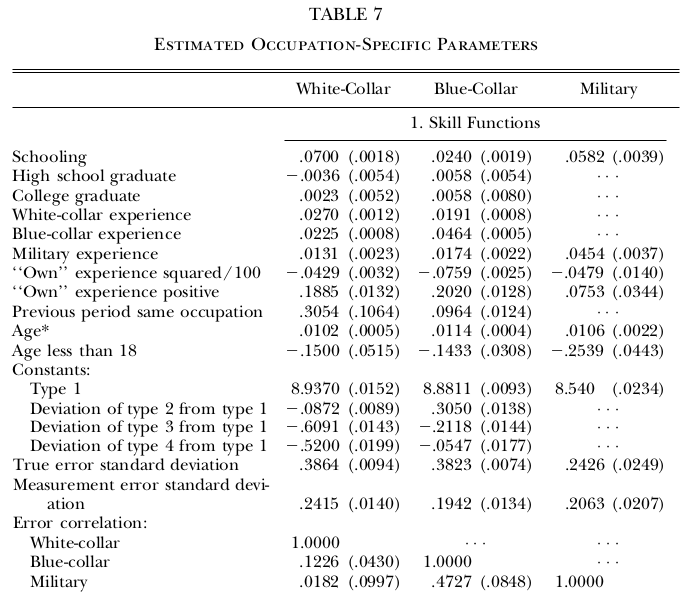
\includegraphics[width=.90\columnwidth]{tab-7}
\end{center}
\end{frame}
%-------------------------------------------------------------------------------
%-------------------------------------------------------------------------------
\begin{frame}[plain]
\begin{center}
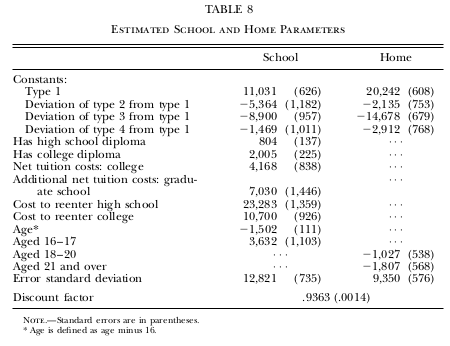
\includegraphics[width=.90\columnwidth]{tab-8}
\end{center}
\end{frame}
%-------------------------------------------------------------------------------
%-------------------------------------------------------------------------------
\begin{frame}[plain]
\begin{center}
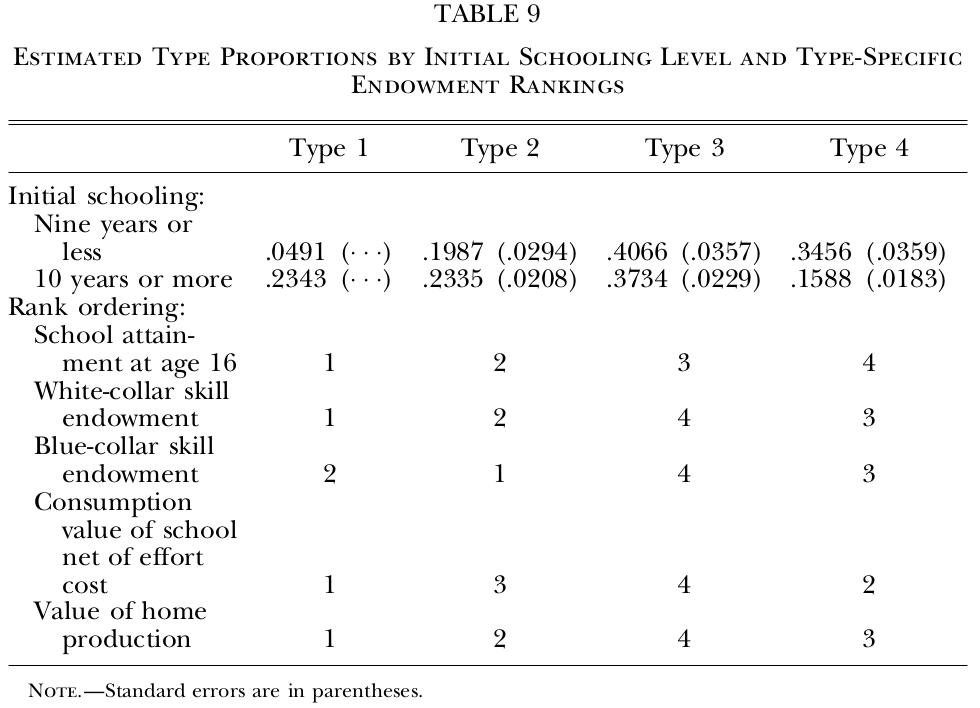
\includegraphics[width=.90\columnwidth]{tab-9}
\end{center}
\end{frame}
%-------------------------------------------------------------------------------
%-------------------------------------------------------------------------------
\begin{frame}[plain]
\begin{center}
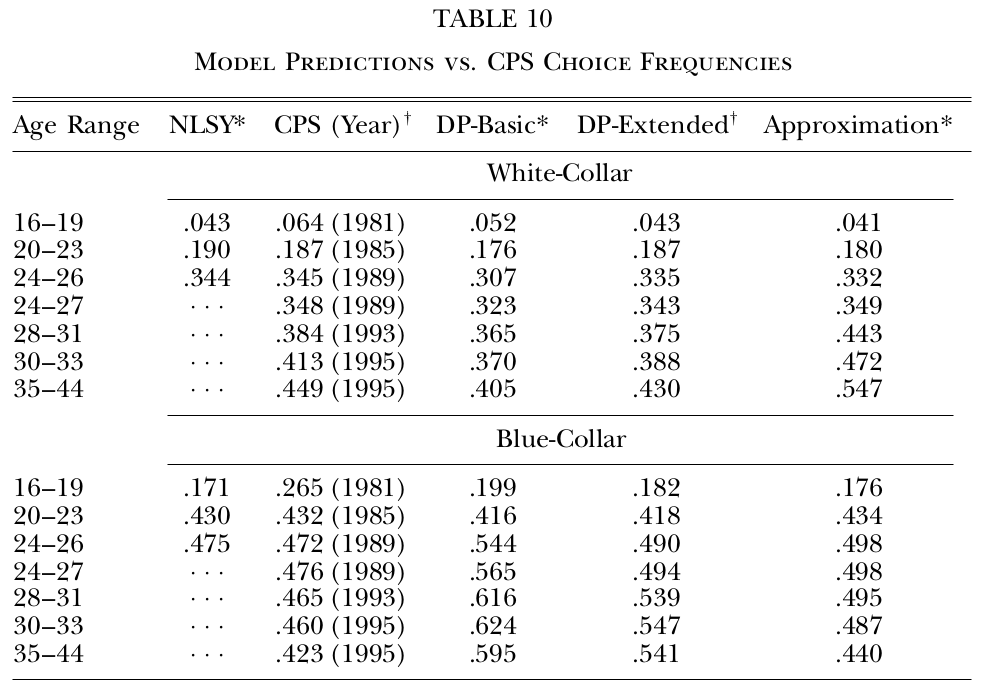
\includegraphics[width=.90\columnwidth]{tab-10}
\end{center}
\end{frame}
%-------------------------------------------------------------------------------
%-------------------------------------------------------------------------------
\begin{frame}[plain]
\begin{center}
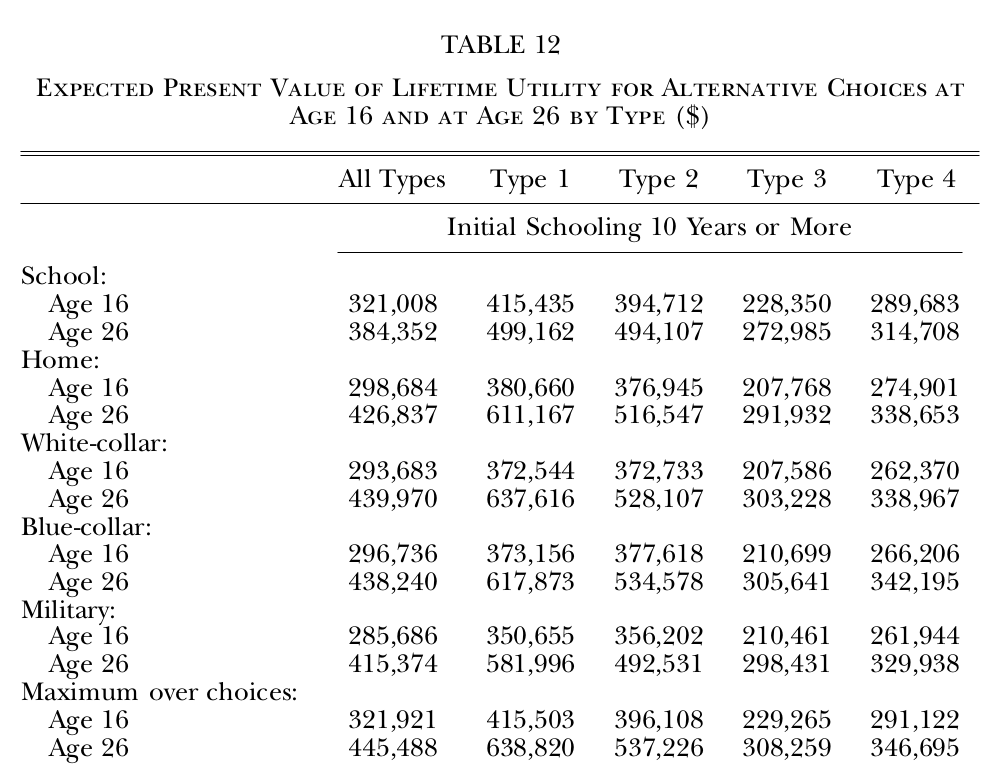
\includegraphics[width=.90\columnwidth]{tab-12}
\end{center}
\end{frame}
%-------------------------------------------------------------------------------
%-------------------------------------------------------------------------------
\begin{frame}\begin{quote}
... skill endowment heterogeneity is potentially an important determinant of inequality in lifetime welfare. Indeed, on the basis of the simulated data, the between-type variance in expected lifetime utility is calculated to account for 90 percent of the total variance. It is especially troublesome, given this finding, that unobserved heterogeneity is usually left as a black box.
\end{quote}\end{frame}
%-------------------------------------------------------------------------------
%-------------------------------------------------------------------------------
\begin{frame}[plain]
\begin{center}
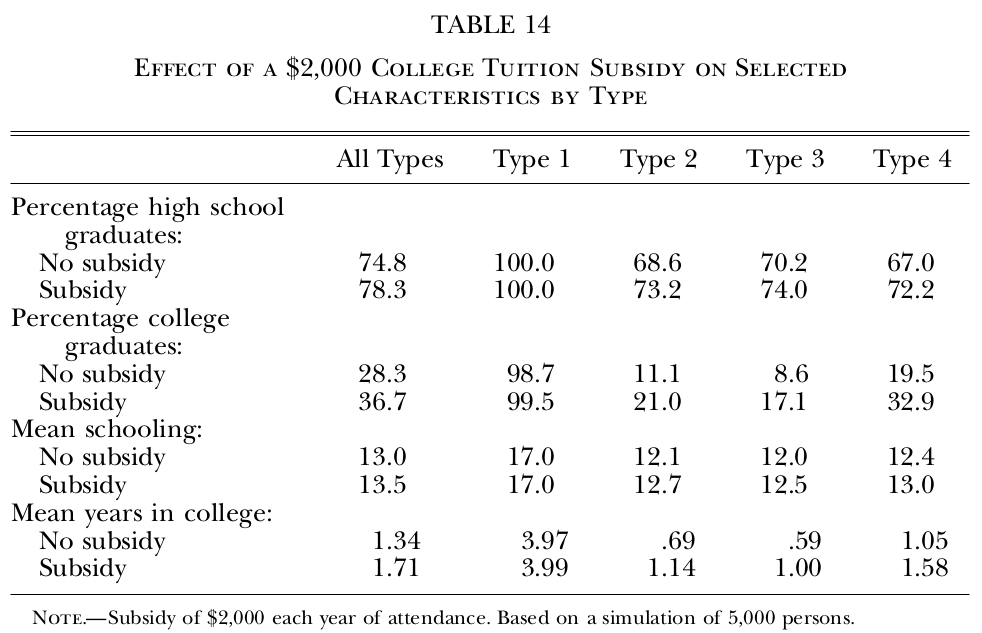
\includegraphics[width=.90\columnwidth]{tab-14}
\end{center}
\end{frame}
%-------------------------------------------------------------------------------
%-------------------------------------------------------------------------------
